\chapter{Аргын тодорхойлолт}

Энэхүү ажлын мөн чанар нь үндсэн судалгаа бөгөөд гэсэн хэдий ч үр дүн, түүнтэй хамт ашиглагдах програм болон санг үүсгэхдээ өөрийн тодорхойлсон дараах шаардлагуудад нийцүүлэн хөгжүүлэхээр зорьсон. Үүнд:

\begin{enumerate}
	\item Өгөгдөл нь цэвэр гараар бичигдсэн ба маш сайн боловсруулагдсан байх \label{criteria:1}
	\item Тэмдэгтийн зургууд дахин давтагдаагүй, мөн тухайн тэмдэгтийн бичигдэж болох аль болох олон хувилбаруудыг агуулсан байх \label{criteria:2}
	\item Тэмдэгтүүд дээр шинэ зургууд нэмж өгөгдлийн хэмжээг томруулах, зөвхөн шаардлагатай тэмдэгтүүдээр өөр шинэ датасет үүсгэх боломжтой байх \label{criteria:3}
	\item Өгөгдлийг аль болох олон төрлөөр авч ашиглах, шаардлагатай статистик мэдээллийг авах боломжтой байх \label{criteria:4}
	\item Өгөгдөл нь өөрөө болон, өгөгдөл үүсгэх программ нь хэнд ч авч ашиглахад нээлттэй байх \label{criteria:5}
\end{enumerate}

\section{Оролт}

Энэхүү судалгааны ажлын оролтын хувьд хүний гараар бичигдсэн крилл үсэг, тоо болон тусгай тэмдэгтүүд байх бөгөөд \textit{Шаардлага №\ref{criteria:1}} -т тэмдэглэсний дагуу өгөгдөл нь цэвэр гараар бичигдсэн ба болосвруулалт сайн хийгдсэн байх ёстой. Тийм ч учраас тоо, том жижиг крилл үсгүүд болон хэд хэдэн тусгай тэмдэгтүүдээс бүрдсэн маягт гаргасан бөгөөд боловсруулалтын үр дүнг хялбаршуулах, өгөгдлийн чанарыг сайжруулах зорилготойгоор хэд хэдэн удаа шинэчилсэн. Зураг \ref{fig:sheets}.
Гэвч тайлангийн энэ хэсэгт ерөнхийдөө маягтын загварууд хэрхэн өөрчлөгдсөн дээр анхаарах бөгөөд яг боловсруулалт, ашигласан арга зэргийг энэ бүлгийн \ref{section:processing} хэсэгт дэлгэрэнгүй авч үзнэ.


\begin{figure}[ht]
	\begin{subfigure}{0.5\textwidth}
		\centering
		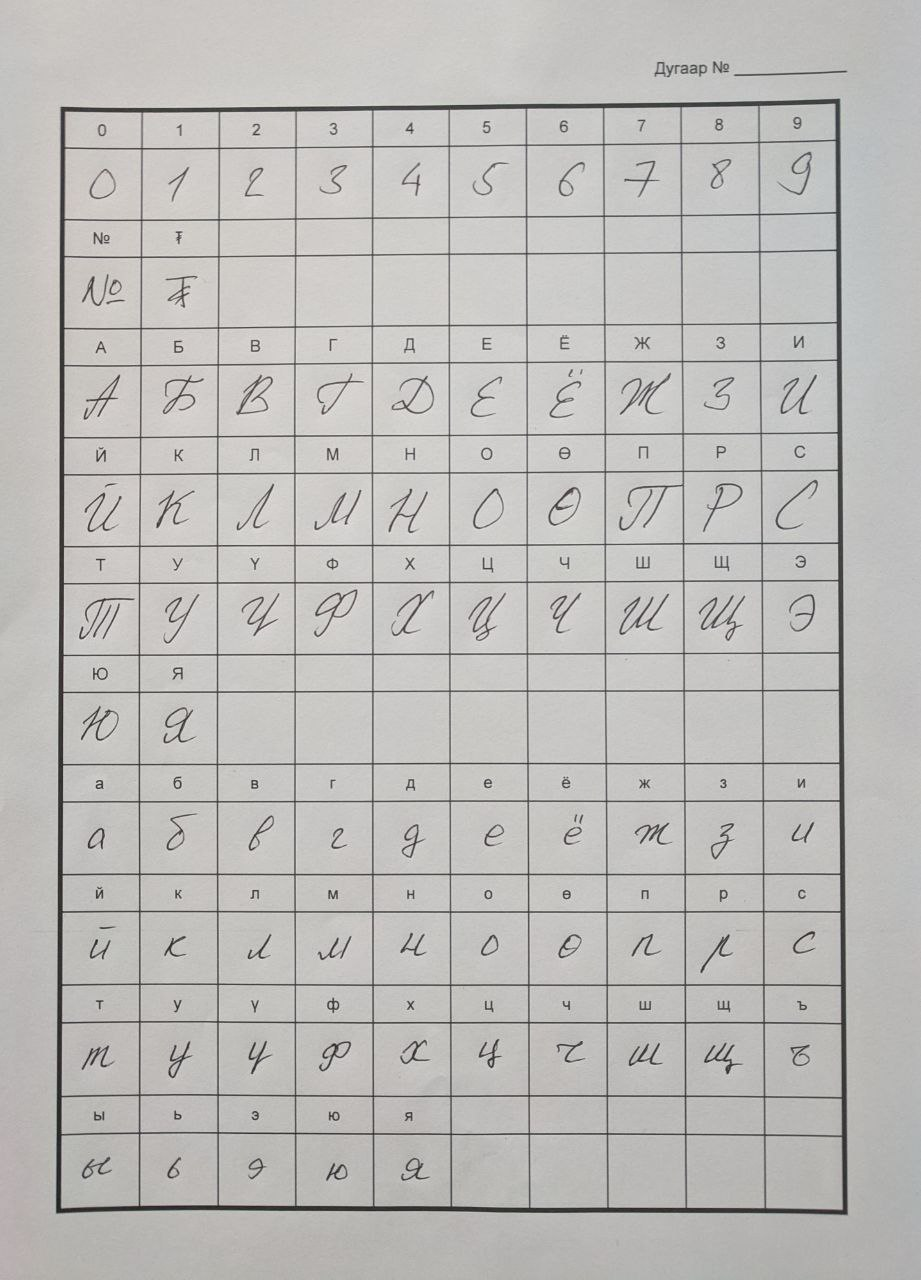
\includegraphics[width=0.9\linewidth]{images/sheet_1}
		\caption{Хамгийн эхний хувилбар}
		\label{fig:sheet_1}
	\end{subfigure}
	\begin{subfigure}{0.52\textwidth}
		\centering
		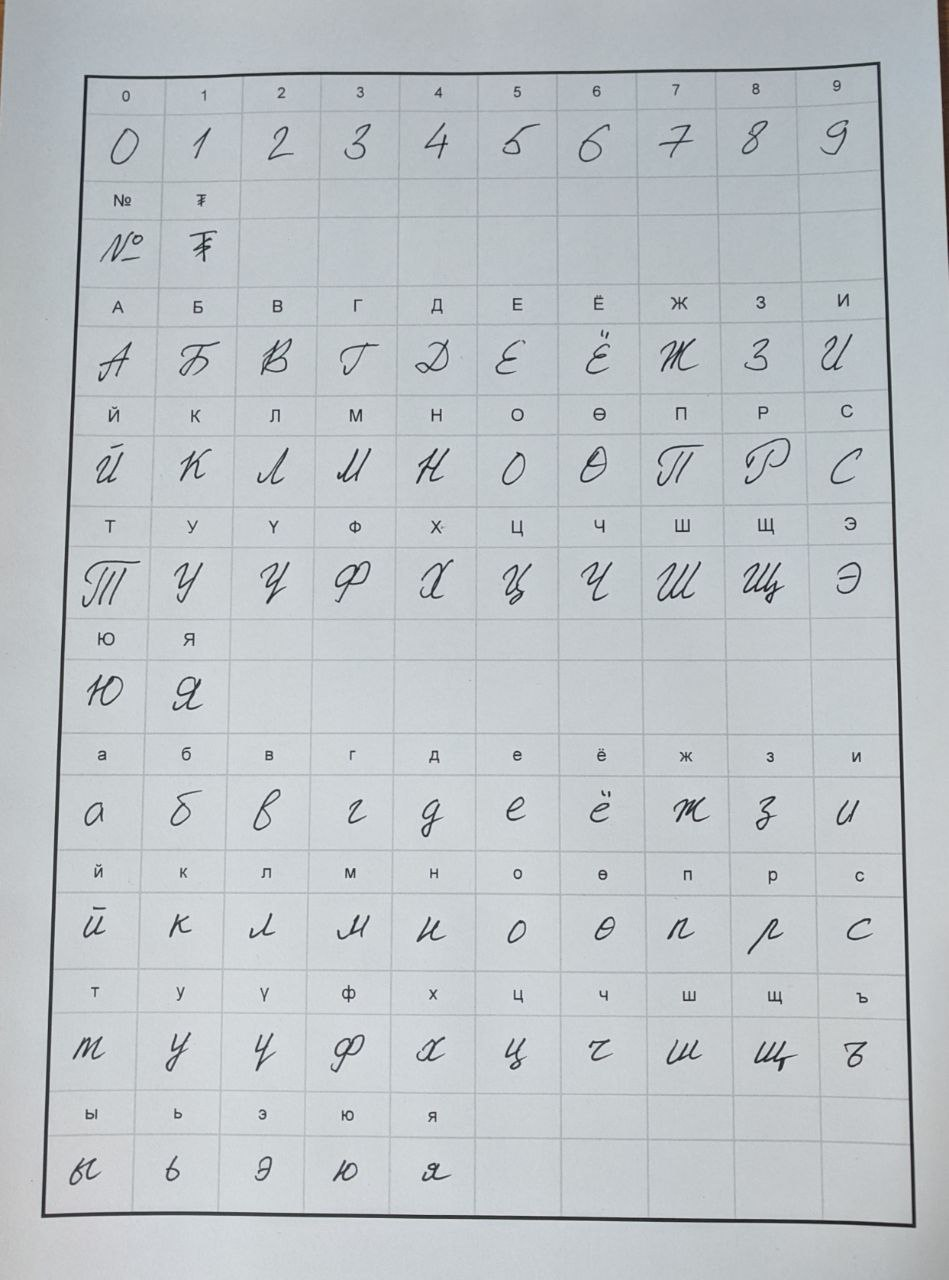
\includegraphics[width=0.9\linewidth]{images/sheet_2}
		\caption{Удаах хувилбар}
		\label{fig:sheet_2}
	\end{subfigure}
	\caption{Өгөгдөл цуглуулахдаа ашиглахаар бэлтгэсэн гар бичмэлийн маягтын хувилбарууд}
	\label{fig:sheets}
\end{figure}


Гэр бичмэлийн маягтыг зураг боловсруулах үед үндсэн бичвэрийг агуулах хүснэгтийг олоход амар байлгах үүднээс зузаан, тод хүрээ оруулсан, харин хүснэгтийн нүднүүдийн хүрээг гадна талын хүрээнээс харьцангуй бүдэг байдлаар бэлтгэсэн хэдий ч боловсруулалтын үед бичвэр агуулж буй хүснэгтээс нүд болгоныг салган авахад Зураг \ref{fig:sheet_1} дээрх хамгийн гадна талын нүднүүдийн хүрээ хэтэрхий тод байсан нь цааш тэмдэгт бүр дээр боловсруулалт хийхэд саад болж байсныг Зураг \ref{fig:sheet_1_segmented}-ээс харж болно. Учир нь зургийг ямар өнцөгөөс дарсан, гэрэл сүүдэр хэрхэн бууснаас хамааран ялангуяа хүснэгтийн захын нүднүүдийн харгалзах талд маш тод зураасууд боловсруулалт хийгдсэний дараа ч үлдсэн байсан.

\begin{figure}[ht]
	\begin{subfigure}{0.5\textwidth}
		\centering
		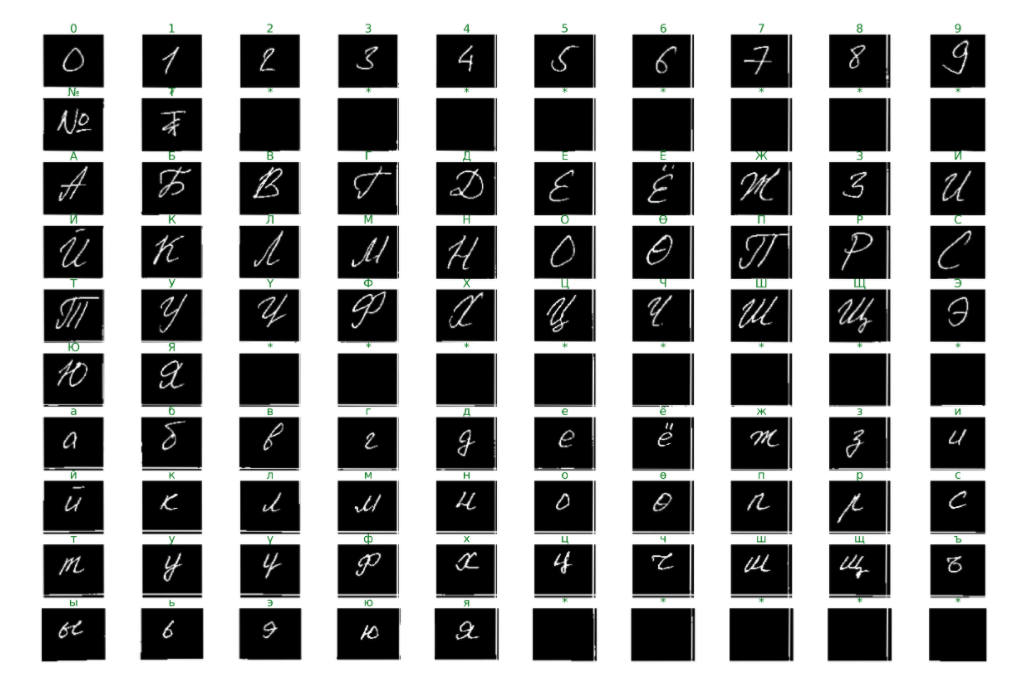
\includegraphics[width=0.9\linewidth]{images/sheet_1_segmented}
		\caption{Хамгийн эхний хувилбарын боловсруулалт}
		\label{fig:sheet_1_segmented}
	\end{subfigure}
	\begin{subfigure}{0.5\textwidth}
		\centering
		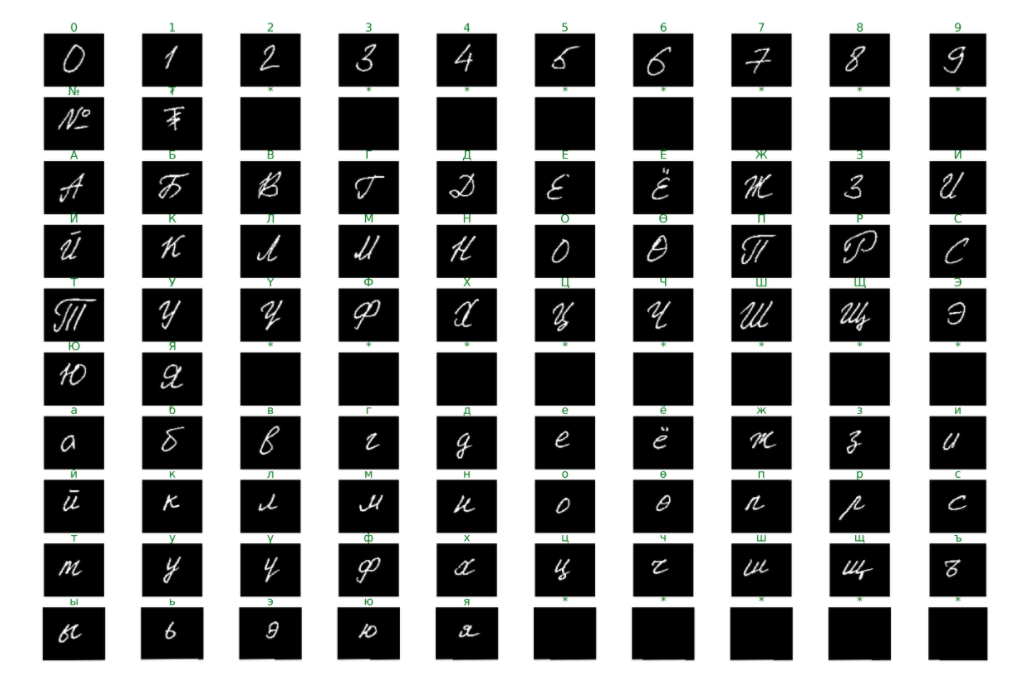
\includegraphics[width=0.9\linewidth]{images/sheet_2_segmented}
		\caption{Удаах хувилбарын боловсруулалт}
		\label{fig:sheet_2_segmented}
	\end{subfigure}
	\caption{Маягтын зургуудыг зураг боловсруулах аргууд ашиглан үндсэн бичвэрийг хадгалж буй хүснэгтийг илрүүлэн, хүснэгтийн нүд бүрийг салган авахад үүссэн үр дүн}
	\label{fig:sheets_cropped}
\end{figure}

Энэ асуудлыг боловсруулалт хийх аргуудаа өөрчлөх, сайжруулах байдлаар шийдэж болох байсан хэдий ч нүдэнд тэмдэгтүүд хэрхэн бөглөгдсөн, зураг ямархуу байдлаар дарагдсан зэргээс хамааран тийм ч тохиромжтой шийдэл болохгүй гэж үзээд үндсэн маягтын загварыг Зураг \ref{fig:sheet_2} -т харагдаж буй болгон өөрчилсөн ба боловсруулалтын үр дүн хэрхэн сайжирсаныг Зураг \ref{fig:sheet_2_segmented} -аас харж болно.

Үүнээс гадна \textit{Шаардлага №\ref{criteria:3}} -т тодорхойлогдсоны дагуу шинээр тэмдэгтүүд нэмэх, өгөгдлийг өргөжүүлэх боломжтой байх ёстой ба үүний тулд оролтын маягтыг зөвхөн крилл үсгүүд, тоо болон хэдхэн тусгай тэмдэгтүүдээр хязгаарлаж болохгүй. Маягтад бөглөгдөх тэмдэгтүүдийг өөрчлөн (жишээ нь: өөр хэл дээр гар бичмэлийн сан үүсгэх) ашиглах боломжтой байлгах үүднээс маягтын загвар үүсгэхдээ дараах зүйлсийг анхаарсан. Үүнд:

\begin{enumerate}
	\item Хүснэгтийн нүд бүрийн хэмжээ адилхан байх --- Учир нь хүснэгтээс тэмдэгтүүдийг ялган авахдаа анх танисан хүснэгтийг маягтын оролтын зурагны файлын нэр дээр тодорхойлогдсон мөр, баганы тоогоор тэнцүү хуваан авч боловсруулж байгаа юм.
	\item Мөр, баганы тоог маягтын файлын нэрэнд хавсаргасан байх --- Програм маягтыг уншаад боловсруулалт хийн тэмдэгтүүдийг олохдоо хүснэгтээс файлын нэрэнд хавсаргасан мөр, баганыг тоог ашиглаж байгаа.
	\item Хүснэгтэд байгаа тэмдэгтүүдийн дараалал зүүнээс баруун, дээрээс доош чиглэлд байх --- Боловсруулалт амжилттай хийгдэж тэмдэгт бүрийг олсон хэдий ч аль нүд яг ямар тэмдэгтийг төлөөлж байгаа гэдгийг мэдэхийн тулд маягт бүр дээр энэ дараалал тодорхой байх ёстой.
\end{enumerate}

Дээрх шаардлагуудад нийцүүлэн санг үүсгэхдээ ашиглах эцсийн хувилбар, гар бичмэлийн маягтын жишээг Зураг \ref{fig:sheet_final}-аас харж болно.

\begin{figure}
	\centering
	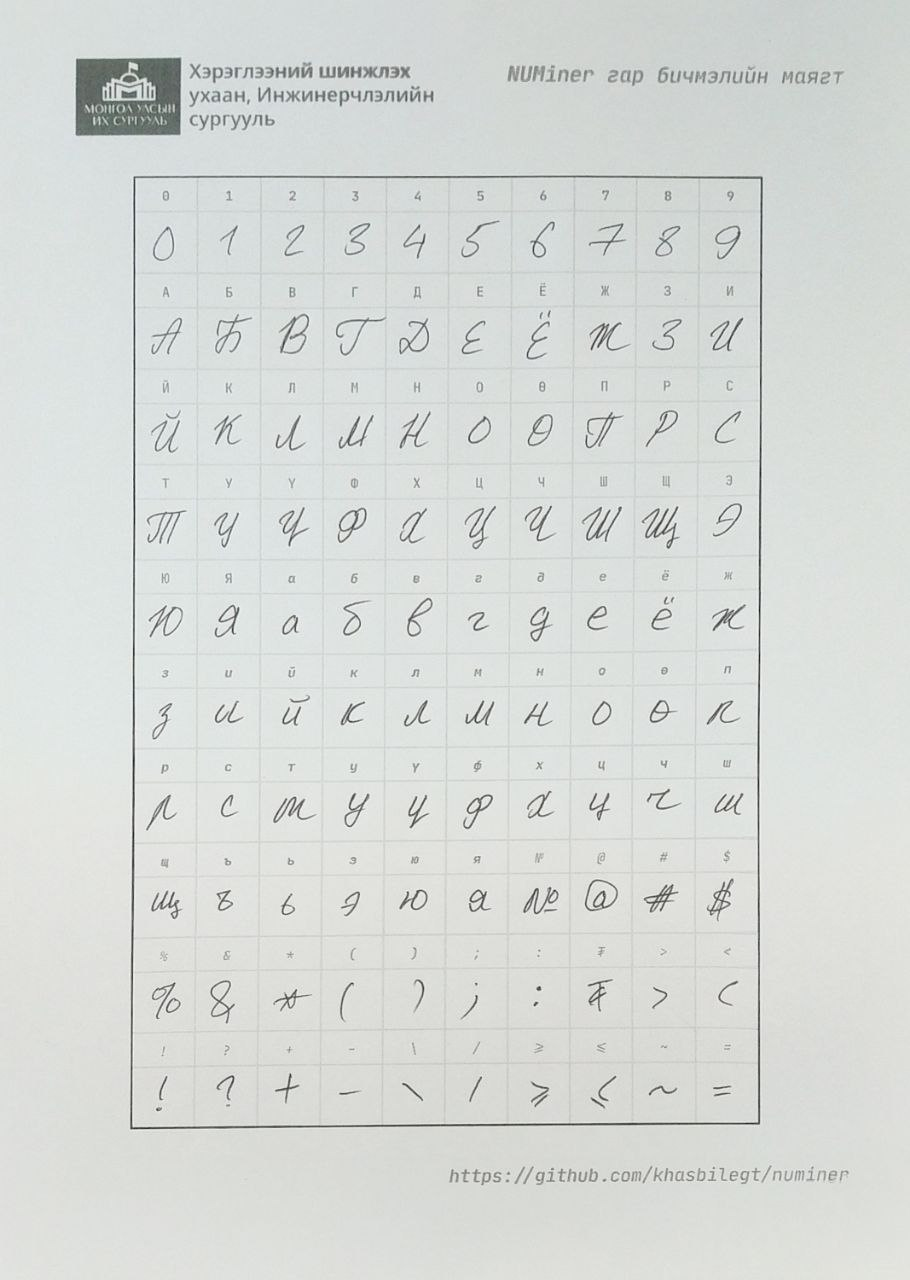
\includegraphics[width=0.6\linewidth]{images/sheet_final}
	\caption{Гар бичмэлийн маягтын хамгийн эцсийн хувилбар}
	\label{fig:sheet_final}
\end{figure}

\section{Боловсруулалт}
\label{section:processing}

Гар бичмэлийн маягтыг бөглүүлэн авсны дараа тухайн маягтын зураг нь оролтын зураг болно. Оролтын зураг дээр тоон зураг боловсруулалт\footnote{Компьютерийн шинжлэх ухаанд, зураг боловсруулалт гэдэг нь тоон хэлбэрийн зургийг, цахим тооцоолуурын тусламжтай тодорхой алгоритмын хүрээнд боловсруулахыг хэлнэ. \cite{image-processing}} -ын аргууд ашиглан тэмдэгт бүрт харгалзах гараар бичигдсэн хэсгүүдийг олох, бичвэр тус бүрт мөн тодорхой боловсруулалт дахин хийх ба ерөнхий байдлаар дараах алхамуудыг гүйцэтгэнэ. Үүнд:

\begin{itemize}
	\item Маягтын зургийг хүн бөглөсөн даруйд сканнердах боломжгүй учир тоон зураг болгохын тулд маягтын зургийг нь дарж оруулж байгаа. Иймээс оролтын зураг тодорхой хэмжээнд шуугиантай, гэрлийн нөлөөлөлд автсан байх магадлалтай хэдий ч бэлдсэн маягтаас, тодорхой шаардлагын дагуу маягтын зургийг аль болох шуугиан багатай, гэрлийн нөлөөгүй авч байгаа. Гэсэн ч энэ нь үр дүн ямар байхад сөргөөр нөлөөлөх учир оролтын зурагнаас шуугиан арилгах, гэрлийн нөлөөг багасгах
	\item Маягт доторх мэдээллүүдээс бидэнд хамгийн хэрэгтэй хэсэг нь тэмдэгтүүд болон бичвэрүүдийг агуулж буй хүснэгт бөгөөд энэхүү хүснэгтийг оролтын зурагны аль хэсэгт байгааг олж мэдэх зорилгоор дөрвөн булангуудыг оролтын зураг дээрээс олох
	\item Маягтыг тоон болгон хөрвүүлэхдээ дийлэнхи тохиолдолд гар утас камерыг ашиглана гэж үзэж байгаа учир өмнөх шатанд илрүүлсэн бичвэр агуулсан хүснэгт нь зураг дээр эгц, тэгш буух нь эргэлзээтэй. Тийм ч учраас оролтын зургаас харах өнцгийн хувиргалтыг арилган, тэгшлэх
	\item Өмнөх шатны үр дүнгээс тэмдэгт болон тухайн тэмдэгтийн гараар бичигдсэн хэсгийг хүснэгтийн мөр, баганы тооноос ялган авах, нүд бүрээс ангилалтай (= label) хэсгийг салгах
	\item Гараар бичигдсэн тэмдэгт тус бүрд гаралтад тодорхойлогдсон шаардлагуудын дагуу дахин боловсруулалт хийх
\end{itemize}

\section{Гаралт}

Энэхүү ажлын \ref{criteria:mnist-compatible} хэсгийг үндэслэн гараар бөглөгдсөн маягтаас ялгасан тэмдэгтүүдийг EMNIST сангийн жишгээр боловсруулахаар шийдсэн.

\begin{itemize}
	\item Зураг нь хоёртын буюу binary зураг байх
	\item Үндсэн тэмдэгтийг багтаасан хамгийн жижиг тэгш өнцөгт авч, 2 пикселийн хүрээ нэмсэн 28х28 пиксел хэмжээтэй байх
\end{itemize}